\newif\ifjapanese
\japanesetrue % 論文全体を日本語で書く(英語で書くならコメントアウト)
\ifjapanese
	\documentclass[11pt]{jreport}
	\renewcommand{\bibname}{参考文献}
	\newcommand{\acknowledgmentname}{謝辞}
\else
	\documentclass[11pt]{report}
	\newcommand{\acknowledgmentname}{Acknowledgment}
\fi

%ページ番号消す
\pagestyle{empty}

%レイアウト確認
%\usepackage{layout}

\usepackage{ascmac}
\usepackage{here}				%図を強制的に出力する
\usepackage{amsmath}			%枠組み・数式用パッケージ
\usepackage{amssymb}			%数式用パッケージ
\usepackage{multirow}			%段組みのためのパッケージ
\usepackage[dvipdfmx]{graphicx} %PDFへのタイプセットのための関数
\usepackage{mathptmx}			%欧文と数式フォントをAdobe Timesに変更
%\usepackage{mediabb}			%貼り込むPDFのxBBファイルを自動生成
\usepackage{exscale}			%大型演算子のスケーリングもしてくれる。
\usepackage{longtable}			%ページをまたぐ表を、きれいに表示
\usepackage{dcolumn}			%表中で小数点揃えをしてくれる。
\usepackage[a4paper]{geometry}	%余白を1ページだけ調整
\usepackage{style/fancyhdr}		%ヘッダーフッターの調整
\usepackage{caption}			%キャプションの設定
%\usepackage{listings,jlisting}	%同梱「jlisteing」読み込み
								% プログラムソースコードを表示する。
%\usepackage[multi,deluxe,bold]{otf}	%OTFフォントの使用(別途mapで設定したものになる)
\usepackage{lscape}              %用紙を横向きにレイアウト
%\usepackage[top=5mm, hmargin=10mm, bottom=25mm]{geometry}
%--------------------------------------------------------------------
\usepackage{style/repo-format}   %同梱の「repo-format.sty」を読込
\usepackage{style/aco-index}     %同梱の「aco-index.sty」を読込
\usepackage{style/roman_math}    %同梱の「roman_math.sty」を読込(ローマ数字)

\begin{document}
\tableofcontents
\pagenumbering{arabic}
\chapter{序論}
\thispagestyle{fancy}
\nobreak
\section{研究背景と目的}
本研究は「オーディトリウムの“底”で演奏を聴く」という旧態依然とした鑑賞形態及びそれに基づく決定論的設計法に対し、建築音響学の観点から新たな息吹を吹き込むことで、次世代の建築を設計するための礎を築こうとするものである。

\subsection{2階バルコニー最前列席の音響的評価}
この世に存在する全てのオーディトリウムは、いずれも室固有の響きを持っており、それは室を構成する形と内装条件によって決定づけられる。一般的な音響設計では、どの客席においても一様な反射音が到達するよう計画される。
ここで、収容人数や舞台へ向けての視野を確保する観点から、オーディトリウムにバルコニー席を設けることが多々ある。このとき、バルコニー先端部は前方に客席がなく、ホール空間へ張り出した特異な場となる。
\\ さて、2階バルコニー最前列の座席は、音響的に高い評価を得ることが多い$^{\text{\cite{01-1}}}$。これは、ホール空間が有する吸音力の大半(500Hzで7割程度)$^{\text{\cite{01-2}}}$を受け持っている1階客席床面(椅子+聴衆の吸音力)から相対的に離れた場所に位置するため、エネルギ減衰の少ない有効な直接音や反射音を得やすいことに起因すると定性的に推察されている(\textgt{図}\ref{fig:2階バルコニー最前列席の音場})。
\\
\\
\begin{figure}[h]
    \centering
    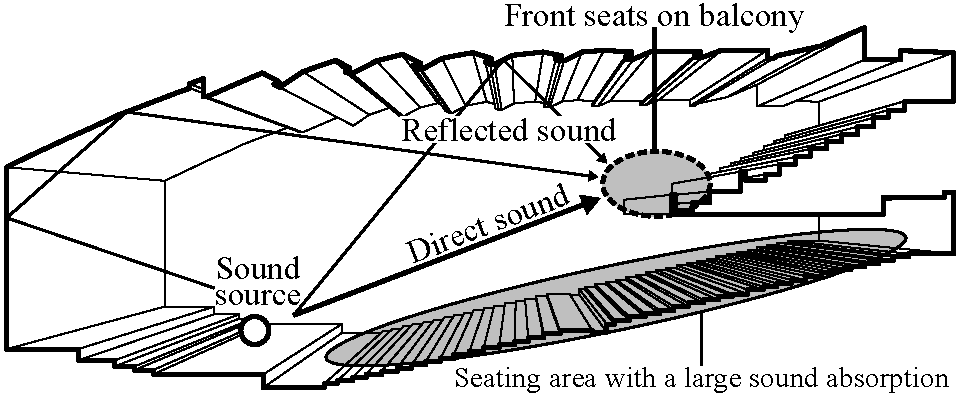
\includegraphics[keepaspectratio,scale=0.8]{01_att/second_balcony.pdf}
    \caption{\hspace{1mm}2階バルコニー最前列席の音場}
    \label{fig:2階バルコニー最前列席の音場}
\end{figure}

%-------------------------------------------------------------
\newpage
\subsection{評価対象領域の拡張}
美しい響きを生み出すにあたり、室容積は人間を収容するには冗長な大きさを要する。規模により異なるものの、室容積から算出されるホールの天井高はおおよそ10$\sim$20mである。ホール空間は人が鑑賞可能なエリアを断面方向含め無数に拡張できるというポテンシャルを秘めているにも関わらず、オーディトリウムの底で鑑賞をするという様式は依然として変わっていない。
\\ 建築音響学が体系化した1900年以後$^{\text{\cite{01-3}}}$、ホールの音響性能について種々研究が行われているものの、音場測定や解析シミュレーションによる音場の評価は、当然のことながら、建築的に確定された客席床面(床面上高さ1$\sim$2m)における面的評価に留まっており、ホール空間全体を評価対象とした設計研究は皆無である。本研究では、前節で述べた知見を踏まえ、評価対象領域を3次元的に拡張した評価を試みる(\textgt{図}\ref{fig:評価対象領域の拡張})。
\\
\begin{figure}[h]
    \centering
    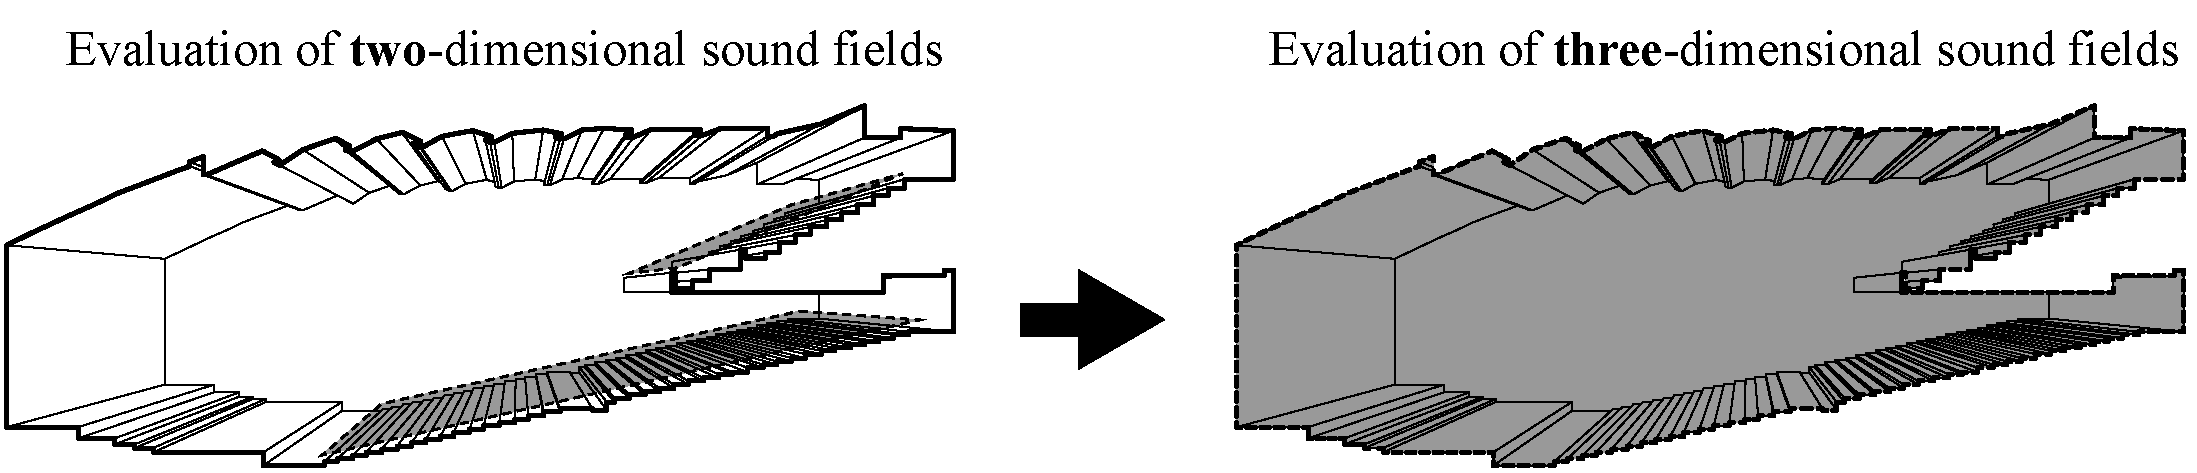
\includegraphics[keepaspectratio,scale=0.41]{01_att/evaluate_area.pdf}
    \caption{\hspace{1mm}評価対象領域の拡張}
    \label{fig:評価対象領域の拡張}
\end{figure}

\subsection{研究目的}
本研究は、コンサートホール音場の評価対象領域を、吸音力の大きな座席面近傍音場から3次元的に拡張し、座席面遠方音場(\textgt{図}\ref{fig:座席面遠方音場})の音響物理特性を明らかにすることにより、従来の面的評価並びにそれに基づく決定論的設計法に新たな可能性を見出すことを目的とするものである。
\\
\begin{figure}[h]
    \centering
    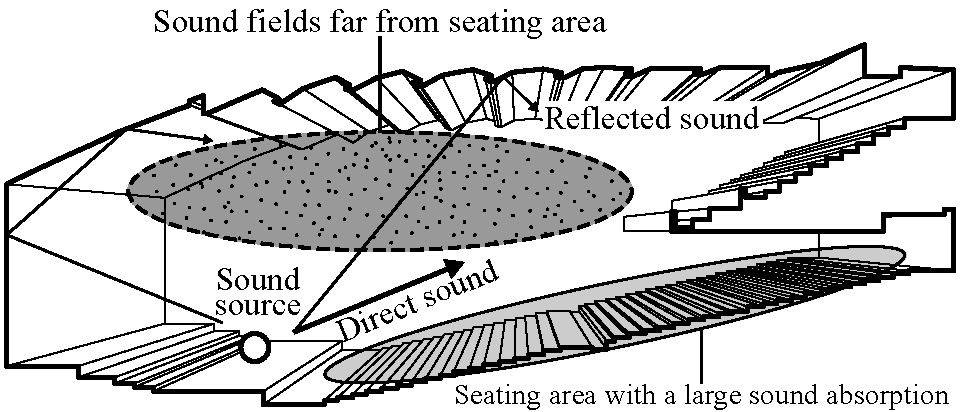
\includegraphics[keepaspectratio,scale=0.8]{01_att/zasekimen_enpo_English.pdf}
    \caption{\hspace{1mm}座席面遠方音場}
    \label{fig:座席面遠方音場}
\end{figure}

%-------------------------------------------------------------
\newpage
\section{既往の研究と本論の位置づけ}
\subsection{音環境の心理評価システム}
物理的特性と聴覚的効果との対応を考える必要があることを説明する
\\→本論文は物理的特性をとりあげた研究であること(聴覚的効果との対応は含まない)を言及する。

\subsection{室内音響物理指標}
4つの要素感覚とそれに対応すると提案されている物理量について説明する。

\subsection{フライングバルコニーを有するホールの事例}
Philharmonie de Parisを例にフライングバルコニーの紹介、本研究のテーマに近いホールがあることを示し、本テーマは突拍子もないことではないことを示す。

\section{論文構成}
本論文は、以下に示す全7章で構成される。
\\ 第1章では前節までに本研究の背景と目的、関連する既往研究の概要、本論の位置づけについて述べた。本節では、論文の構成について述べている。
\\ 第2章では、研究手法である幾何音響解析の概要、解析条件並びに解析モデルについて述べる。
\\ 第3章では、解析で得られたデータから残響特性の観点から音場評価を行う。
\\ 第4章では、時間エネルギ特性の観点から音場評価を行う。
\\ 第5章では、反射音方向分布特性の観点から距離減衰特性及び方向別エネルギ率の観点から音場評価を行う。
\\ 第6章では、これまでの研究結果を踏まえ、ホール形状の設計例を提示する。
\\ 最後の第7章では、本論文の結論を述べる。

\chapter{空間全体を対象とした幾何音響解析}

\section{幾何音響解析手法について}
幾何音響解析手法とは、音の波動としての性質を無視して、その伝搬を幾何的に取り扱う手法のことである$^{\text{\cite{02-5}}}$。非常に直感的で理解しやすい方法であり、あまり多くの計算機資源を必要とせず、計算時間も波動音響解析手法と比べ短いため、大規模空間を扱う際の現実的手法として広く用いられている。厳密な予測が必要となる詳細設計の段階では音響縮尺模型実験や波動音響解析に頼らざるを得ないが、基本計画段階における検討や初期反射音構造の予測等に対しては大変有用であると考えられている。
幾何音響学に基づいた代表的なコンピュータシミュレーション手法として、音線法と鏡像法が挙げられる(\textgt{図}\ref{fig:音線法と鏡像法})。
\\ 音線法(Ray-tracing method)とは、音源から等立体間隔で多数の音線を出すことで、反射伝搬経路を追跡計算する手法であり、距離減衰は音線間の広がり(音線の密度)によって考慮される。なお、有限の間隔で放射された音線が丁度受音点を通過することは極めて稀なため、有限の大きさを持つ受音領域を設けることが一般的である。しかしながら、受音点が領域を持つゆえに同一経路の反射音が重複したり、現実にはない反射経路を抽出したり等の計算誤差が生じる。この問題を解決するため、複数のアルゴリズムが考案されている$^{\text{\cite{02-6}}}$。
\\ 鏡像法(Image source method)は周壁各面における音源の鏡像を幾何学的に求め、各鏡像から受音点までの経路を求める手法である。距離減衰と通った反射面の吸音率からインパルス応答を近似的に求めることができるが、反射次数の増加とともに鏡像の数が指数関数的に増加するため、高次の反射音まで求めることは困難である$^{\text{\cite{02-5}}}$。
\\ 音線法と鏡像法のいずれも、初期反射音の検討に対して非常に有用であると考えられるが、拡散反射を考慮できない幾何音響シミュレーションのみでは、反射回数が増加するに従い、現実の音場との誤差が大きくなってしまう。そこで近年では乱反射率(Scattering coefficient)などの導入により、室内音場の長時間のインパルス応答を求めようとする試みがある。

\begin{figure}[H]
    \centering
    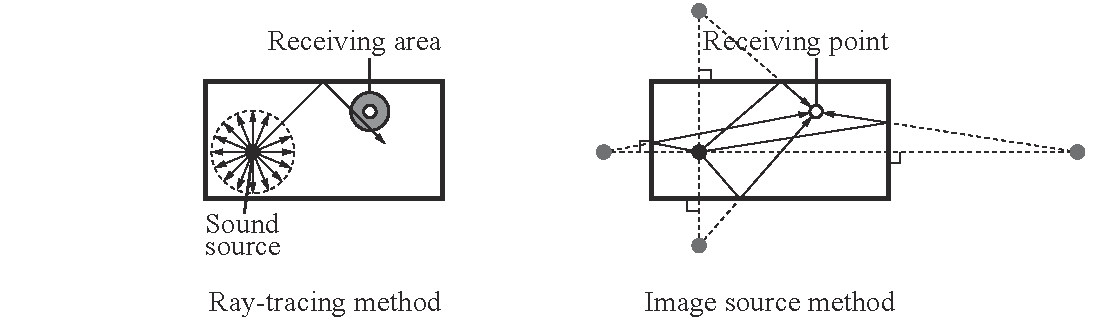
\includegraphics[keepaspectratio,scale=0.8]{02_att/kikaonkyo.pdf}
    \caption{\hspace{1mm}音線法と鏡像法の概念図}
    \label{fig:音線法と鏡像法}
\end{figure}

\section{解析条件}
本研究で用いる幾何音響解析ソフトには3つの解析タイプ(Audio area mapping, Early part detailed, Full detailed calculation)があり、それぞれ音線法、鏡像法、Randomized Tail-corrected Cone-tracing method (RTC)により計算される(\textgt{表}\ref{3つの解析タイプ})。
RTCとは音線の先に円の有限領域をもたせるCone-tracingと標準的な音線法及び鏡像法をハイブリッドした解析手法である。
\\ 本研究ではこれらのうち、後期反射音までのインパルス応答を算出するFull detailed calculationから室内音響物理指標を、9次反射音までのインパルス応答(方向情報含む)[\textgt{図}\ref{fig:Early_IR}]を算出するEarly part detailedから方向別物理量を各々求めた。解析条件を解析タイプ別に\textgt{表}\ref{Full_set}と\textgt{表}\ref{Early_set}に示す。
\\
% 3つの解析手法について
\begin{table}[htbp]
\centering
\caption{解析手法と出力データ}
\label{3つの解析タイプ}
\resizebox{\textwidth}{!}{%
\begin{tabular}{ccccc}
\Hline
Type & Prediction methods & \multicolumn{3}{c}{Output data} \\ \cline{3-5} 
 &  & \multicolumn{2}{c}{Impulse response} & Room acoustic parameters \\ \cline{3-4}
 &  & \multicolumn{1}{c|}{Time domain} & Spatial information &  \\ \hline
Audio area mapping & Ray-tracing method & $\times$ & $\times$ & $\bigcirc$ \\
Early part detailed & Image source method & Early part only & $\bigcirc$ & $\times$ \\
Full detailed calculation & RTC method & Full & $\bigtriangleup^{*}$ & $\bigcirc$ \\ \Hline
\multicolumn{5}{l}{$^{*}$ : limited spatial information}
\end{tabular}%
}
\end{table}

\begin{figure}[htbp]
    \centering
    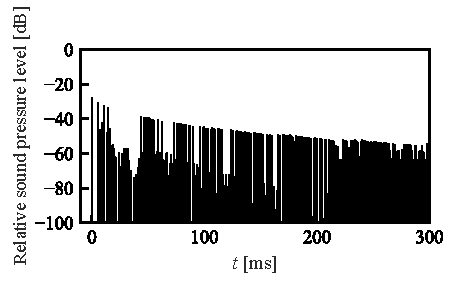
\includegraphics[keepaspectratio,scale=1]{02_att/Early_IR.pdf}
    \caption{\hspace{1mm}Early part detailedにより算出されたインパルス応答}
    \label{fig:Early_IR}
\end{figure}

%EarlyとFullの解析条件
\begin{table}[htbp]
\begin{minipage}[t]{.45\textwidth}
    \begin{center}
    \caption{Full detailed calculationの解析条件}
    \label{Full_set}
      \begin{tabular}{lc}%ひだり
      \Hline
      \multicolumn{1}{c}{Setting items} & Input value \\ \hline
      Number of rays & 99,9999 \\
      Truncation time [ms] & 3,500 \\ \Hline
      \end{tabular}
    \end{center}
  \end{minipage}
  %
  \hfill
  %
  \begin{minipage}[t]{.45\textwidth}
    \begin{center}
    \caption{Early part detailedの解析条件}
    \label{Early_set}
      \begin{tabular}{lc}%みぎ
      \Hline
      \multicolumn{1}{c}{Setting items} & \multicolumn{1}{c}{Input value} \\ \hline
      Specular reflection order (0-9) & 9 \\
      Diffuse reflection order (0-1) & 1 \\
      Truncation time [ms] & 300 \\ \Hline
      \end{tabular}
    \end{center}
  \end{minipage}
\end{table}

\pagebreak
また、音速と空気吸収は\textgt{式}\ref{eq:speed_of_sound}と\textgt{式}\ref{eq:air_absorption}により定められる。本研究では一般的な室内を想定し、$\theta$=20[{\kern-.2em\r{}\kern-.3em C}]、$\phi=50[\%]$とした。すなわち、$c=343$[m/s]、 $m_b=0.63\times10^{-3}$[m$^{-1}$](500Hz)の条件下で解析を行った。

\begin{equation}
 \label{eq:speed_of_sound}
c = 331.4\sqrt{1+\frac{\theta}{273}}
\end{equation}
\begin{equation}
 \label{eq:air_absorption}
m_b = \mathrm{from \; ISO \; 9613.1^{\text{\cite{organizacion1993iso}}} \; based \; on \; \theta, \; f_b, \; and \; \phi}
\end{equation}
\hspace{2cm}$\theta$ : air temperature, {\kern-.2em\r{}\kern-.3em C}\\
\hspace{2cm}$m_b$ : air dissipation coefficient, m$^{-1}$\\
\hspace{2cm}$f_b$ : octave-band center frequency, Hz\\
\hspace{2cm}$\phi$ : relative humidity, $\%$

\section{解析モデル}
解析モデルは収容人員1,500人程度のコンサートホールを想定し、平面形状が矩形のモデル(TypeA)と扇形のモデル(TypeB)の2種類の空間モデルを対象とした。両モデルとも舞台高さを1m、奥行きを10mに統一した。
\\ 観測点は客席床面上と上部空間の音場性能を比較するために2m\(\times\)2m\(\times\)2mの格子状に(A)矩形モデルで840点、(B)扇形モデルで712点設けた。
また、音線が音源方向から到来したときに反射音到来角度が\(0^\circ\)になるよう、観測点の座標系を設定した。
音源は無指向性音源を舞台中央に高さ1.5mとした。両ホールの音響諸元を\textgt{表}\ref{解析モデルの音響諸元}に示す。
%%%%%%%%%%%%%%%%%%%
\begin{table}[htbp]
\centering
\caption{解析モデルの音響諸元}
\label{解析モデルの音響諸元}
\begin{tabular}{lccccc}
\Hline
\multicolumn{1}{c}{Type} & \textit{V}{[}m$^3${]} & \textit{V}/\textit{S}{[}m{]} & \textit{RT}$^{*1}${[}s{]} &$\bar{\alpha}$& N$^{*2}$ \\ \hline
(A)Rectanglular & 15,268 & 3.8 & 2.2 & 0.24 & 840 \\
(B)Fan-shape & 15,329 & 3.8 & 2.2 & 0.24 & 712 \\ \Hline
\multicolumn{6}{l}{$^{*1}$ : calculated with Eyring-Knudsen formula (500Hz)} \\
\multicolumn{4}{l}{$^{*2}$ : N indicates the number of receiving points}
\end{tabular}
\end{table}
%%%%%%%%%%%%%%%%%%%

\subsection{形状の設計}
現存するホールを参考$^{\text{\cite{02-1}}}$に(A)矩形モデル及び(B)扇形モデルの設計を行った。
両ホールの断面図及び平面図を\textgt{図}\ref{fig:(A)矩形モデル及び(B)扇形モデル断面図}と\textgt{図}\ref{fig:(A)矩形モデル及び(B)扇形モデル平面図}に示す。

\newpage
%-------------------------------------------------------------------------
\begin{figure}[H]
    \centering
    \includegraphics[keepaspectratio,scale=0.99]{02_att/rec_fan_zumen_1.pdf}
    \caption{\hspace{1mm}(A)矩形モデル及び(B)扇形モデル断面図}
    \label{fig:(A)矩形モデル及び(B)扇形モデル断面図}
\end{figure}

\begin{figure}[H]
    \centering
    \includegraphics[keepaspectratio,scale=0.99]{02_att/rec_fan_zumen_2.pdf}
    \caption{\hspace{1mm}(A)矩形モデル及び(B)扇形モデル平面図}
    \label{fig:(A)矩形モデル及び(B)扇形モデル平面図}
\end{figure}

\subsection{吸音率の設定}
室の内装面は客席床と後壁を吸音性、その他の面を反射性とし、両ホールの残響時間が等しくなるように現実的な吸音率(250$\sim$2kHz)$^{\text{\cite{01-3}\cite{02-1}\cite{02-2}}}$を設定した。客席床の吸音率については国内の標準的な1席(人+モケット張り椅子)の吸音力$^{\text{\cite{02-4}}}$を1席あたりの床面積(=0.6m$^2$)で除した値(\textgt{表}\ref{客席面の吸音率})を用いた。解析モデルに用いた吸音率を\textgt{表}\ref{解析モデルの吸音率}に示す。
\\
\\
%%%%%%%%%%%%%%%%%%%
\begin{table}[htbp]
\begin{center}
\caption{客席面の(a)吸音力と(b)吸音率}
\label{客席面の吸音率}
\begin{tabular}{llcccccc}
\Hline
&&\multicolumn{6}{c}{Frequency{[}Hz{]}}\\\cline{3-8}
&&125&250&500&1k&2k&4k\\\hline
(a)&\begin{tabular}[c]{@{}l@{}}Sound absorption of a seat \\(human and moquette-clad chair) \end{tabular}&0.23&0.32&0.40&0.43&0.43&0.41\\\hline
(b)&\begin{tabular}[c]{@{}l@{}}Sound absorption coefficient \\equivalent to (a)\end{tabular}&0.38&0.53&0.67&0.72&0.72&0.68\\\Hline
\end{tabular}
\end{center}
\end{table}
%%%%%%%%%%%%%%%%%%%
\\
\\
%%%%%%%%%%%%%%%%%%%
\begin{table}[htbp]
\centering
\caption{解析モデルの吸音率}
\label{解析モデルの吸音率}
\resizebox{\textwidth}{!}{%
\begin{tabular}{llcccccc}
\Hline
                         &                                           & \multicolumn{6}{c}{Frequency{[}Hz{]}}   \\ \cline{3-8} 
\multicolumn{1}{c}{Site} & \multicolumn{1}{c}{Material}              & 125  & 250  & 500  & 1k   & 2k   & 4k   \\ \hline
Ceiling \_ main floor    & Plaster board (12mm) with large air space & 0.25 & 0.15 & 0.10 & 0.08 & 0.06 & 0.05 \\
Ceiling \_ stage         & Acoustic reflector                        & 0.15 & 0.15 & 0.10 & 0.08 & 0.07 & 0.06 \\
Floor \_ main floor      & Human and moquette-clad chair             & 0.38 & 0.53 & 0.67 & 0.72 & 0.72 & 0.68 \\
Floor \_ stage           & Floor joist of stage (45mm)               & 0.15 & 0.10 & 0.08 & 0.07 & 0.05 & 0.05 \\
Side wall \_ main floor  & Concrete                                  & 0.01 & 0.02 & 0.02 & 0.03 & 0.03 & 0.03 \\
Rear wall \_ main floor  & Glass wool (25mm) with large air space    & 0.55 & 0.80 & 0.75 & 0.48 & 0.33 & 0.15 \\
Wall \_ stage            & Acoustic reflector                        & 0.15 & 0.15 & 0.10 & 0.08 & 0.07 & 0.06 \\ \Hline
\end{tabular}%
}
\end{table}
%%%%%%%%%%%%%%%%%%%
\pagebreak
\subsection{乱反射率の設定}
乱反射率(Scattering coefficient)はISO17497-1$^{\text{\cite{iso2004acoustics}}}$の中で壁面の全反射エネルギーに対する鏡面反射成分以外のエネルギーの割合として定義され、\textgt{式}\ref{eq:scatter}で表される。ここで$E_{total}$は全反射エネルギー、$E_{spec}$は鏡面反射エネルギーである。


\begin{equation}
 \label{eq:scatter}
s_{\theta}=1-\frac{E_{spec}}{E_{total}}
\end{equation}

\vspace{0.8cm}

解析では、周波数に応じて座席部に0.3$\sim$0.7を、それ以外の面に0.1を与えた$^{\text{\cite{02-3}}}$。
解析モデルに用いた乱反射率を\textgt{表}\ref{解析モデルの乱反射率}に示す。\\
 また、壁面隅角部における音の散乱(端部散乱)を考慮した乱反射率を与える研究$^{\text{\cite{02-7}}}$が進められている。
壁面端部から$\lambda$/8分の面積を1、それ以外の面積を0として面積平均した乱反射率を吸音面の接合面に与えたときに実測との対応が良くなることが既往の研究$^{\text{\cite{02-8}}}$から明らかになっているが、これは本研究で使用する幾何音響解析ソフトの端部散乱を考慮した乱反射率(壁面端部から$\lambda$/4分の面積を0.5、それ以外の面積を0として面積平均したもの(\textgt{式}\ref{eq:付加乱反射率計算式}、\textgt{図}\ref{fig:壁面端部}))に近似する。
解析モデルにおいて端部散乱を考慮した面を\textgt{表}\ref{端部散乱を適用する面}に示す。

\vspace{0.8cm}

%%%%%%%%%%%%%%%%%%%
\begin{table}[htbp]
\centering
\caption{解析モデルの乱反射率}
\label{解析モデルの乱反射率}
\resizebox{\textwidth}{!}{%
\begin{tabular}{llcccccc}
\Hline
&& \multicolumn{6}{c}{Frequency{[}Hz{]}}   \\ \cline{3-8} 
\multicolumn{1}{c}{Site} & \multicolumn{1}{c}{Material}              & 125  & 250  & 500  & 1k   & 2k   & 4k   \\ \hline
Ceiling \_ main floor    & Plaster board (12mm) with large air space & 0.10 & 0.10 & 0.10 & 0.10 & 0.10 & 0.10 \\
Ceiling \_ stage         & Acoustic reflector                        & 0.10 & 0.10 & 0.10 & 0.10 & 0.10 & 0.10 \\
Floor \_ main floor      & Human and moquette-clad chair             & 0.30 & 0.40 & 0.50 & 0.60 & 0.70 & 0.80 \\
Floor \_ stage           & Floor joist of stage (45mm)               & 0.10 & 0.10 & 0.10 & 0.10 & 0.10 & 0.10 \\
Side wall \_ main floor  & Concrete                                  & 0.10 & 0.10 & 0.10 & 0.10 & 0.10 & 0.10 \\
Rear wall \_ main floor  & Glass wool (25mm) with large air space    & 0.10 & 0.10 & 0.10 & 0.10 & 0.10 & 0.10 \\
Wall \_ stage            & Acoustic reflector                        & 0.10 & 0.10 & 0.10 & 0.10 & 0.10 & 0.10 \\ \Hline
\end{tabular}%
}
\end{table}
%%%%%%%%%%%%%%%%%%%

\vspace{0.8cm}

\begin{table}[htbp]
\begin{equation}
 \label{eq:付加乱反射率計算式}
 s_{\scalebox{0.5}{effective}} = s_{\scalebox{0.5}{surface}} + \frac{s_{\scalebox{0.5}{edge}}
 S_{\scalebox{0.5}{edge}}}{S_{\scalebox{0.5}{surface}}}\\
\end{equation}
\hspace{2cm}$s_{\scalebox{0.5}{edge}} = 0.5$\\
\hspace{2cm}$s_{\scalebox{0.5}{surface}}$ : The normal surface scattering coefficient\\
\hspace{2cm}$S_{\scalebox{0.5}{edge}}$ : The area of an edge quarter of a wavelength wide\\
\hspace{2cm}$S_{\scalebox{0.5}{surface}}$ : The complete plane or sub-plane area\\
\end{table}

\begin{figure}[htbp]
    \centering
    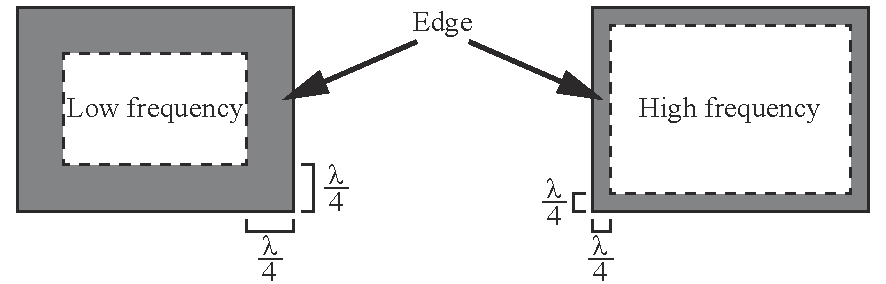
\includegraphics[keepaspectratio,scale=0.8]{02_att/edge.pdf}
    \caption{\hspace{1mm}壁面端部から$\lambda$/4分の面積}
    \label{fig:壁面端部}
\end{figure}

%%%%%%%%%%%%%%%%%%%
\begin{table}[htbp]
\centering
\caption{端部散乱を考慮する面}
\label{端部散乱を適用する面}
\begin{tabular}{llc}
\Hline
\multicolumn{1}{c}{Site} & \multicolumn{1}{c}{Type} & Apply edge diffusion to surface \\ \hline
Ceiling \_ main floor    & Reflective               & *                               \\
Ceiling \_ stage         & Reflective               & *                               \\
Floor \_ main floor      & Absorptive               &                                 \\
Floor \_ stage           & Reflective               & *                               \\
Side wall \_ main floor  & Reflective               & *                               \\
Rear wall \_ main floor  & Absorptive               &                                 \\
Wall \_ stage            & Reflective               & *                               \\ \Hline
\end{tabular}
\end{table}
%%%%%%%%%%%%%%%%%%%

\chapter{評価手法}
\section{一元配置分散分析}
残響時間は正規分布に従うため、一元配置分散分析を行う。
\section{共分散分析}
EDTを観測高さごとに比較するため、ノンパラメトリック分散分析を行う。
\chapter{音圧レベル特性評価}
\chapter{反射音方向分布特性}

\section{反射音の方向情報}
反射音の方向情報をみるため、解析で得られたインパルス応答から鉛直方向成分、側方成分、前後方向成分に分解した。なお、反射音の到来角度は音源方向を$0^\circ$とした。
\\ 初期反射音($t$=0$\sim$80[ms])の側方成分は観測高さによる違いは見られないものの、鉛直方向成分は座席面遠方音場($H$=14.0)において豊富に到来しているのに対し、座席面近傍音場($H$=1.2)では著しく不足していることが読み取れる。

\includepdf[pages=-, angle=90]{05_att/ir_rec3.pdf}

\section{反射音方向別エネルギ比}
ここで、反射音の到来方向バランスを定量的に把握するため、初期反射音の全エネルギ($t$=0$\sim$80[ms])に対する鉛直方向成分の割合$ER_V$(vertical energy ratio)、側方成分の割合$ER_L$(lateral energy ratio)、前後方向成分の割合$ER_G$(longitudinal energy ratio)を各々算出した(\textbf{式}\ref{eq:ERV}$\sim$\ref{eq:ERG})。ここで$\delta$は仰角(鉛直上方向:0$^\circ$)、$\theta$は水平角(側方:0$^\circ$)を表す。

\begin{table}[htbp]
\begin{equation}
  \label{eq:ERV}
  ER_V = {\frac{\displaystyle\int_0^{80}p^2(t)cos^2{\delta}dt}{\displaystyle\int_0^{80}p^2(t)dt}} 
\end{equation}

\begin{equation}
  \label{eq:ERL}
  ER_L = {\frac{\displaystyle\int_0^{80}p^2(t)sin^2{\delta}cos^2{\theta}dt}{\displaystyle\int_0^{80}p^2(t)dt}} 
\end{equation}

\begin{equation}
  \label{eq:ERG}
  ER_G = {\frac{\displaystyle\int_0^{80}p^2(t)sin^2{\delta}sin^2{\theta}dt}{\displaystyle\int_0^{80}p^2(t)dt}} 
\end{equation}

\centering
\includegraphics[keepaspectratio,scale=1]{04_att/direction.png}
\label{fig:}
\end{table}

\pagebreak
\section{$DUI$の導入}
ここで鉛直方向・側方・前後方向から反射音エネルギが均等に到来するとき、$ER_V$、$ER_L$、$ER_G$の3値は全て$\frac{1}{3}$となることから、反射音の到来方向に関する空間バランスを見るための指標として3次元直交座標系における点($ER_V$,$ER_L$,$ER_G$)と点($\frac{1}{3}$,$\frac{1}{3}$,$\frac{1}{3}$)の距離$d_i$を観測点ごとに求め(\textbf{式}\ref{eq:di})、その空間内全観測点の平均値として$DUI$(Directional Uniformity Index)$^{\text{\cite{後期音}}}$を算出する(\textbf{式}\ref{eq:DUI})。以後、$DUI$を用いて反射音到来方向分布の一様度の評価を行う。
\begin{table}[htbp]
\begin{equation}
  \label{eq:di}
  d_i = \sqrt{\left({ER_V-\frac{1}{3}}\right)^2 + \left(ER_L-\frac{1}{3}\right)^2 + \left(ER_G-\frac{1}{3}\right)^2} 
\end{equation}
\begin{equation}
    \label{eq:DUI}
    DUI=\frac{\sum_{i=1}^N{d_i}}{N}
\end{equation}
\end{table}

\pagebreak
\section{観測点の座標系について}
反射音方向分布特性をみるにあたり、観測点における座標系の置き方について2通りの検討を行った(\figref{observing})。\\
(i)観測点の座標系を解析モデルの3次元直交座標系にあわせる(正面:y軸負の方向)\\
(ii)観測点の座標系を音源中心の極座標系にする(正面:音源)\\
(i),(ii)それぞれの場合の$ER_V$、$ER_L$、$ER_G$及び$d_i$の分布を観測高さ$H$[m]ごとに示す。

\begin{figure}[htbp]
    \centering
    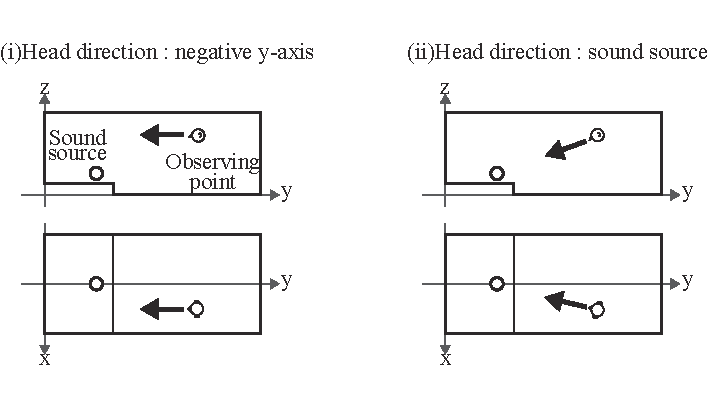
\includegraphics[keepaspectratio,scale=1]{05_att/observing.pdf}
    \caption{\hspace{1mm}\textbf{Study of head direction}}
    \label{fig:observing}
\end{figure}

\includepdf[pages=-]{05_att/cont_y.pdf}
\includepdf[pages=-]{05_att/cont_s.pdf}

\subsubsection{(i)正面:y軸負の方向の場合}
天井付近では天井からの反射音が豊富に到来するが、座席部前方では前後方向成分が多くなり、座席後方では鉛直方向成分が多くなる。
すなわち、観測高さ$H$が高い音場では座席部前方で$ER_V$が、座席部後方で$ER_G$が大きな値をとっている(\figref{er_reason})。
一方、$ER_L$が音源付近で高い値をとっている。これは、頭の方向が常にy軸負の方向を向いているため、両耳方向に音源からの直接音が到来し、側方成分が多くなったと考えられる。
\\
\begin{figure}[htbp]
    \centering
    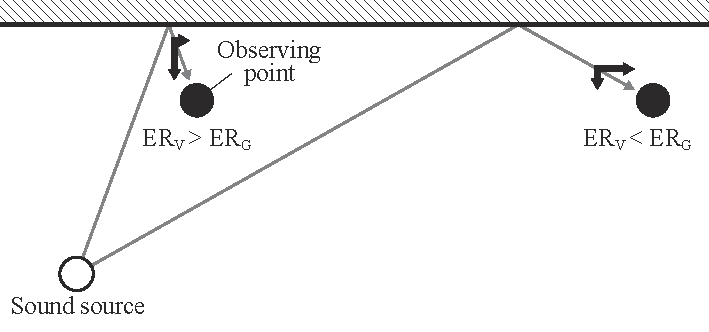
\includegraphics[keepaspectratio,scale=1]{05_att/er_reason.pdf}
    \caption{\hspace{1mm}\textbf{$ER_V$ vs $ER_G$}}
    \label{fig:er_reason}
\end{figure}

\subsubsection{(ii)正面:音源方向の場合}
常に頭が音源を向いているため、直接音は常に前後方向成分に含まれる。$ER_V$、$ER_L$、$ER_G$の和は常に1であるから、$ER_V$と$ER_L$に比べ$ER_G$が全体的に高い値をとっている。側壁付近で$ER_L$が高い値をとっているが、これは頭が音源を向いているため、両耳方向と側壁からの反射音の入射角が合うためであると考えられる。
\\ 本研究では実際にコンサートホールで音を聴いたときに受ける印象と反射音方向分布に符合する(ii)頭の向きを音源としたときの条件で解析を行う。
\pagebreak

\section{観測高さの違いと反射音方向分布特性の分析}


\section{客席面吸音率の変化と反射音方向分布特性の分析}


このとき、$t_A$を最初の反射音が到達するまでの時間、$p_A(t)$を音源からの距離が10mの観測点における直接音の音圧とする。

\begin{equation}
  \label{eq:}
  G_{early} = 10\log_{10}{\frac{\displaystyle\int_0^{80}p^2(t)dt}{\displaystyle\int_0^{t_A}p_{A}^2(t)dt}} \dB
\end{equation}

\begin{equation}
  \label{eq:}
  VG_{early} = 10\log_{10}{\frac{\displaystyle\int_0^{80}p^2(t)cos^2{\delta}dt}{\displaystyle\int_0^{t_A}p_{A}^2(t)dt}} \dB
\end{equation}

\begin{equation}
  \label{eq:}
  LG_{early} = 10\log_{10}{\frac{\displaystyle\int_0^{80}p^2(t)sin^2{\delta}cos^2{\theta}dt}{\displaystyle\int_0^{t_A}p_{A}^2(t)dt}} \dB
\end{equation}

\begin{equation}
  \label{eq:}
  GG_{early} = 10\log_{10}{\frac{\displaystyle\int_0^{80}p^2(t)sin^2{\delta}sin^2{\theta}dt}{\displaystyle\int_0^{t_A}p_{A}^2(t)dt}} \dB
\end{equation}


\chapter{時間エネルギ特性評価}

\chapter{結論}
評価対象領域を拡張することにより、オーディトリウム空間全体の音場特性を拡散性の観点から考察した。その結果、座席面遠方音場は近傍に比べ音響エネルギ分布及び反射音到来方向分布が一様であり、より拡散した音場であることがわかった。これらの結果は「オーディトリウムの“底”で演奏を聴く」という旧態依然とした鑑賞形態に対し座席面遠方音場での鑑賞が最適音場の実現に寄与することを示唆しており、新たなホール空間を設計するための可能性を示すものである。

%******** 付 属 品 **********************************
\begin{acknowledgment}
\thispagestyle{fancy}
%本論文は筆者が芝浦工業大学工学部建築学科古屋研究室在学中に行った研究をまとめたものです。
\\この1年間、ご指導ご高配を賜りました芝浦工業大学教授・古屋浩先生に厚くお礼申し上げます。
先生には研究の進め方から物事に取り組む姿勢、資料の表現方法に至るまで終始厳しくも優しい御指導を賜りました。また、研究に関する御指導だけでなく、日頃の研究室活動においても常に温かいご配慮をいただきました。
「工学的に建築を捉える」というテーマに向かって、これまで研究指導して下さいましたことに重ねて御礼申し上げます。
\\ 古屋研究室の先輩である藤田鋭志さん、原彩乃さん、平舘勇馬さんには研究の具体的なアドバイスから資料の作り方に至るまで多くの御助言をいただきました。ここに記して感謝申し上げます。
\\ 苦楽を共にした同期の黒瀬彰君、清水大世君、染野紗結美さん、田代知樹君、中田絢乃さん、堀野量子さんには公私にわたり本当にお世話になりました。同期の皆様には研究の相談に乗っていただいただけでなく、日々の活動においても多大な御協力を戴きました。心より感謝申し上げます。
\\ 最後に、私がこうして卒業研究に取り組めるよう、いつも支援して下さる両親へ深く感謝いたします。
\\
\begin{flushright}
2019年1月29日\\
松崎 広夢
\end{flushright}
\end{acknowledgment}
	% 謝辞。要独自コマンド、include先参照のこと
\addcontentsline{toc}{chapter}{参考文献}
\bibliographystyle{junsrt}
\bibliography{93_bibliography}% 参考文献。要独自コマンド、include先参照のこと
\appendix
\chapter{解析モデルの形状入力データ}
\section{矩形モデル}
\section{扇形モデル}
\section{客席下に空間を付加したモデル}
\chapter{解析モデルの方向別インパルス応答}


\chapter{解析に用いたプログラムコード}
\section{インパルス応答等のグラフプロット}
\section{距離減衰特性算出プログラム}
\section{反射音方向分布特性算出プログラム}		% 付録

%%******** 空 白 ペ ー ジ(今偶数pgの場合)***************
%\ifodd \arabic{page}
%\else
  \thispagestyle{empty}
  \mbox{}
  \newpage
  \clearpage
%\fi


\begin{landscape}
\begin{figure}[htpb]
  \centering
    \begin{tabular}{cccc}
%----- y = sin(x) -----
      \begin{minipage}{0.25\linewidth}
        \centering
          \includegraphics[keepaspectratio,width=\linewidth,angle=0]
                          {rec_source/80contD_1_2m.png}
      \end{minipage}
%----- y = sin(2x) -----
      \begin{minipage}{0.25\linewidth}
        \centering
          \includegraphics[keepaspectratio,width=\linewidth,angle=0]
                          {rec_source/80contD_1_2m.pdf}
      \end{minipage}
%----- y = sin(3x) -----
      \begin{minipage}{0.25\linewidth}
        \centering
          \includegraphics[keepaspectratio,width=\linewidth,angle=0]
                          {rec_source/80contD_1_2m.pdf}
      \end{minipage}
%----- y = sin(4x) -----
      \begin{minipage}{0.25\linewidth}
        \centering
          \includegraphics[keepaspectratio,width=\linewidth,angle=0]
                          {rec_source/80contD_1_2m.pdf}
       \end{minipage}
    \end{tabular}
\end{figure}
%\layout{} %レイアウトの様子を
\end{landscape}

\end{document}